\documentclass{ximera}
\graphicspath{  %% When looking for images,
{./}            %% look here first,
{./pictures/}   %% then look for a pictures folder,
{../pictures/}  %% which may be a directory up.
{../../pictures/}  %% which may be a directory up.
{../../../pictures/}  %% which may be a directory up.
{../../../../pictures/}  %% which may be a directory up.
}

\usepackage{listings}
%\usepackage{circuitikz}
\usepackage{xcolor}
\usepackage{amsmath,amsthm}
\usepackage{subcaption}
\usepackage{graphicx}
\usepackage{tikz}
%\usepackage{tikz-3dplot}
\usepackage{amsfonts}
%\usepackage{mdframed} % For framing content
%\usepackage{tikz-cd}

  \renewcommand{\vector}[1]{\left\langle #1\right\rangle}
  \newcommand{\arrowvec}[1]{{\overset{\rightharpoonup}{#1}}}
  \newcommand{\ro}{\texttt{R}}%% row operation
  \newcommand{\dotp}{\bullet}%% dot product
  \renewcommand{\l}{\ell}
  \let\defaultAnswerFormat\answerFormatBoxed
  \usetikzlibrary{calc,bending}
  \tikzset{>=stealth}
  




%make a maroon color
\definecolor{maroon}{RGB}{128,0,0}
%make a dark blue color
\definecolor{darkblue}{RGB}{0,0,139}
%define the color fourier0 to be the maroon color
\definecolor{fourier0}{RGB}{128,0,0}
%define the color fourier1 to be the dark blue color
\definecolor{fourier1}{RGB}{0,0,139}
%define the color fourier 1t to be the light blue color
\definecolor{fourier1t}{RGB}{173,216,230}
%define the color fourier2 to be the dark green color
\definecolor{fourier2}{RGB}{0,100,0}
%define teh color fourier2t to be the light green color
\definecolor{fourier2t}{RGB}{144,238,144}
%define the color fourier3 to be the dark purple color
\definecolor{fourier3}{RGB}{128,0,128}
%define the color fourier3t to be the light purple color
\definecolor{fourier3t}{RGB}{221,160,221}
%define the color fourier0t to be the red color
\definecolor{fourier0t}{RGB}{255,0,0}
%define the color fourier4 to be the orange color
\definecolor{fourier4}{RGB}{255,165,0}
%define the color fourier4t to be the darker orange color
\definecolor{fourier4t}{RGB}{255,215,0}
%define the color fourier5 to be the yellow color
\definecolor{fourier5}{RGB}{255,255,0}
%define the color fourier5t to be the darker yellow color
\definecolor{fourier5t}{RGB}{255,255,100}
%define the color fourier6 to be the green color
\definecolor{fourier6}{RGB}{0,128,0}
%define the color fourier6t to be the darker green color
\definecolor{fourier6t}{RGB}{0,255,0}

%New commands for this doc for errors in copying
\newcommand{\eigenvar}{\lambda}
%\newcommand{\vect}[1]{\mathbf{#1}}
\renewcommand{\th}{^{\text{th}}}
\newcommand{\st}{^{\text{st}}}
\newcommand{\nd}{^{\text{nd}}}
\newcommand{\rd}{^{\text{rd}}}
\newcommand{\paren}[1]{\left(#1\right)}
\newcommand{\abs}[1]{\left|#1\right|}
\newcommand{\R}{\mathbb{R}}
\newcommand{\C}{\mathbb{C}}
\newcommand{\Hilb}{\mathbb{H}}
\newcommand{\qq}[1]{\text{#1}}
\newcommand{\Z}{\mathbb{Z}}
\newcommand{\N}{\mathbb{N}}
\newcommand{\q}[1]{\text{``#1''}}
%\newcommand{\mat}[1]{\begin{bmatrix}#1\end{bmatrix}}
\newcommand{\rref}{\text{reduced row echelon form}}
\newcommand{\ef}{\text{echelon form}}
\newcommand{\ohm}{\Omega}
\newcommand{\volt}{\text{V}}
\newcommand{\amp}{\text{A}}
\newcommand{\Seq}{\textbf{Seq}}
\newcommand{\Poly}{\textbf{P}}
\renewcommand{\quad}{\text{    }}
\newcommand{\roweq}{\simeq}
\newcommand{\rowop}{\simeq}
\newcommand{\rowswap}{\leftrightarrow}
\newcommand{\Mat}{\textbf{M}}
\newcommand{\Func}{\textbf{Func}}
\newcommand{\Hw}{\textbf{Hamming weight}}
\newcommand{\Hd}{\textbf{Hamming distance}}
\newcommand{\rank}{\text{rank}}
\newcommand{\longvect}[1]{\overrightarrow{#1}}
% Define the circled command
\newcommand{\circled}[1]{%
  \tikz[baseline=(char.base)]{
    \node[shape=circle,draw,inner sep=2pt,red,fill=red!20,text=black] (char) {#1};}%
}

% Define custom command \strikeh that just puts red text on the 2nd argument
\newcommand{\strikeh}[2]{\textcolor{red}{#2}}

% Define custom command \strikev that just puts red text on the 2nd argument
\newcommand{\strikev}[2]{\textcolor{red}{#2}}

%more new commands for this doc for errors in copying
\newcommand{\SI}{\text{SI}}
\newcommand{\kg}{\text{kg}}
\newcommand{\m}{\text{m}}
\newcommand{\s}{\text{s}}
\newcommand{\norm}[1]{\left\|#1\right\|}
\newcommand{\col}{\text{col}}
\newcommand{\sspan}{\text{span}}
\newcommand{\proj}{\text{proj}}
\newcommand{\set}[1]{\left\{#1\right\}}
\newcommand{\degC}{^\circ\text{C}}
\newcommand{\centroid}[1]{\overline{#1}}
\newcommand{\dotprod}{\boldsymbol{\cdot}}
%\newcommand{\coord}[1]{\begin{bmatrix}#1\end{bmatrix}}
\newcommand{\iprod}[1]{\langle #1 \rangle}
\newcommand{\adjoint}{^{*}}
\newcommand{\conjugate}[1]{\overline{#1}}
\newcommand{\eigenvarA}{\lambda}
\newcommand{\eigenvarB}{\mu}
\newcommand{\orth}{\perp}
\newcommand{\bigbracket}[1]{\left[#1\right]}
\newcommand{\textiff}{\text{ if and only if }}
\newcommand{\adj}{\text{adj}}
\newcommand{\ijth}{\emph{ij}^\text{th}}
\newcommand{\minor}[2]{M_{#2}}
\newcommand{\cofactor}{\text{C}}
\newcommand{\shift}{\textbf{shift}}
\newcommand{\startmat}[1]{
  \left[\begin{array}{#1}
}
\newcommand{\stopmat}{\end{array}\right]}
%a command to give a name to explorations and hints and theorems
\newcommand{\name}[1]{\begin{centering}\textbf{#1}\end{centering}}
\newcommand{\vect}[1]{\vec{#1}}
\newcommand{\dfn}[1]{\textbf{#1}}
\newcommand{\transpose}{\mathsf{T}}
\newcommand{\mtlb}[2][black]{\texttt{\textcolor{#1}{#2}}}
\newcommand{\RR}{\mathbb{R}} % Real numbers
\newcommand{\id}{\text{id}}
\newcommand{\coord}[1]{\langle#1\rangle}
\newcommand{\RREF}{\text{RREF}}
\newcommand{\Null}{\text{Null}}
\newcommand{\Nullity}{\text{Nullity}}
\newcommand{\Rank}{\text{Rank}}
\newcommand{\Col}{\text{Col}}
\newcommand{\Ef}{\text{EF}}
\newcommand{\boxprod}[3]{\abs{(#1\times#2)\cdot#3}}

\author{Zack Reed}
%borrowed from ximera interactive la
\title{Determinants and Geometry}
\begin{document}
\begin{abstract}

\end{abstract}
\maketitle


\section*{Determinants, Areas, and Volumes}

So far, we've focused much of this chapter on determining properties of matrices and specifically whether or not they are invertible. 

We now introduce a very related topic that also has farther reaching implications for matrices as well, beyond invertibility, and is an important measure for Chapters 7, 8, and 9.

An intuition we've been discussing for whether matrices are invertibile is that when linear transformations ``squish'' space down to a smaller dimension, they are not invertible. One way to determine whether this ``squishing'' occurs is to measure by how much units of volume are stretched or compressed through the transformation. 

Consider, for instance, the matrix $\begin{bmatrix}
  3&0&0\\0&2&0\\0&0&1
\end{bmatrix}$. This stretches the $x$-axis by a factor of $3$ and the $y$-axis by a factor of $2$, as you can see in the following GeoGebra applet. Check the ``Adjust Matrix'' box and enter the columns of the matrix accordingly (note that the column vectors are listed as rows when being entered, so really you're entering the transpose of the matrix).

\begin{center}
  \geogebra{mdes5d4h}{858}{509}
\end{center}

As you can see, $A$ stretches out vectors in both the $x$ and $y$ directions while preserving the height. More importantly, the original $1\times1\times1$ cube becomes a stretched out rectangle, and the ``Transformed Volume'' measure reads as $6$. This means that the transformation stretches out space by a factor of $6$. 

If instead you enter the mug-squishing matrix $A=\begin{bmatrix}
  1&0&1\\0&2&2\\1&2&3
\end{bmatrix}$, you see the original cube squished down into a plane. 

The transformed volume of the unit cube is thus $\answer{0}$.

This gives us a clear way to determine whether linear transformations are invertible! Measuring this transformed volume is called finding \emph{the determinant}. The determinant arises from systematically extending the notions of areas and volumes to give clear ways of measuring volume-stretching and volume-compressing for any matrix transformation.


    \subsection*{$2\times 2$ Determinant and the Area of a Parallelogram}
     
    Consider the parallelogram determined by vectors $\vec{u}$ and $\vec{v}$ in $\RR^3$.
     
    \begin{center}
    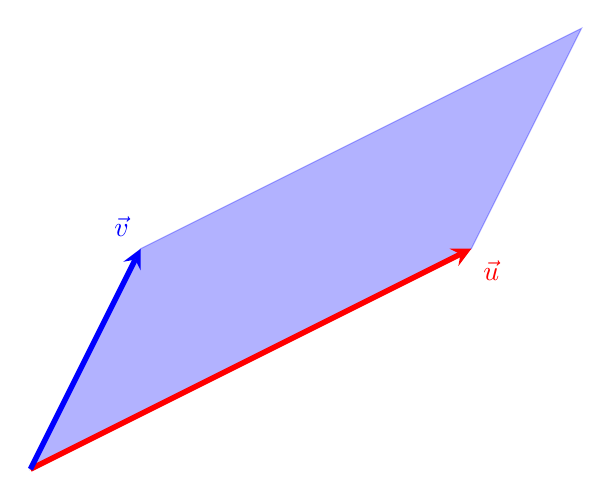
\begin{tikzpicture}[scale=1.4]
     
      \filldraw[blue, opacity=0.3](0,0)--(4,2)--(5,4)--(1,2)--cycle;
     
    \draw[line width=2pt,red,-stealth](0,0)--(4,2) node[below right]{$\vec{u}$};
      
      \draw[line width=2pt,blue, -stealth](0,0)--(1,2) node[above left]{$\vec{v}$};
    \end{tikzpicture}
    \end{center}
     
    Recall that the area of a parallelogram is given by the product of the length of the base and the height.
    As shown in the diagram below, the length of the base is the magnitude of $\vec{u}$. The height, $h$, can be found using trigonometry $$h=\norm{\vec{v}}\sin\theta$$
    \begin{center}
    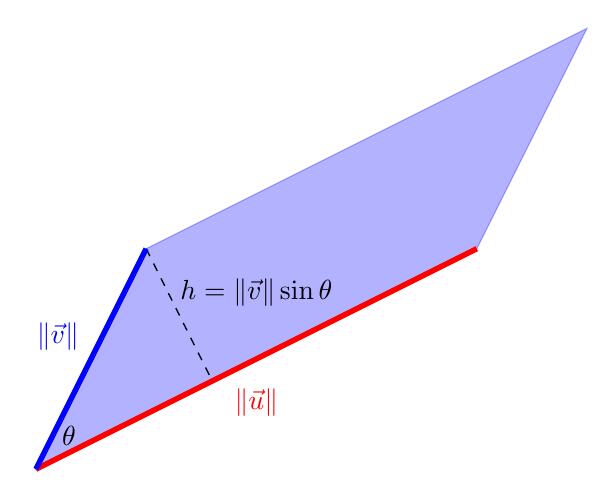
\begin{tikzpicture}[scale=1.4]
     
      \filldraw[blue, opacity=0.3](0,0)--(4,2)--(5,4)--(1,2)--cycle;
     
    \draw[line width=0.5pt, dashed](1,2)--(1.6,0.8);
    \node[] at (2, 1.6)   (b) {$h=\norm{\vec{v}}\sin\theta$};
    \draw[line width=2pt,red](0,0)--(4,2);
     \node[red] at (2, 0.6)   (b) {$\norm{\vec{u}}$};
     \node[blue] at (0.2, 1.2)   (b) {$\norm{\vec{v}}$};
     \node[] at (0.3, 0.3)   (b) {$\theta$};
      \draw[line width=2pt,blue](0,0)--(1,2);
    \end{tikzpicture}
    \end{center}
    Using the area of a parallelogram formula together with Theorem \ref{th:crossproductsin} we get
    $$\mbox{Area}=(\text{base})(\text{height})=\norm{\vec{u}}h=\norm{\vec{u}}\norm{\vec{v}}\sin\theta=\norm{\vec{u}\times\vec{v}}$$
    We have established the following formula.
     
    \begin{formula}\label{form:areaofparallelogram} The area of a parallelogram determined by vectors $\vec{u}$ and $\vec{v}$ in $\RR^3$ is given by
    $$\mbox{Area}=\norm{\vec{u}\times\vec{v}}$$
    \end{formula}
     
    \begin{example}\label{ex:areaOfParFormula}
        Use Formula \ref{form:areaofparallelogram} to find the area of a parallelogram determined by vectors
        $$\vec{u}=\begin{bmatrix}-2\\1\\3\end{bmatrix},\quad \vec{v}=\begin{bmatrix}1\\6\\2\end{bmatrix}$$
    \begin{explanation}
        We can start by visualizeing the parallelogram in GeoGebra.  RIGHT-CLICK and DRAG to rotate the image below.  The area of the parallelogram, rounded to two decimal places, is displayed inside the parallelogram.
     
    \pdfOnly{
    Access GeoGebra interactives through the online version of this text at
     
    \href{https://ximera.osu.edu/oerlinalg}{https://ximera.osu.edu/oerlinalg}.
    }
     
     
    \begin{onlineOnly}   
    \begin{center}
    \geogebra{g7g6kjqm}{600}{400}
    \end{center}
    \end{onlineOnly}
     
        To find the exact area we compute
        $$\vec{u}\times \vec{v}=\begin{bmatrix}-2\\1\\3\end{bmatrix}\times \begin{bmatrix}1\\6\\2\end{bmatrix}=\begin{vmatrix}\vec{i} &\vec{j} &\vec{k}\\-2 & 1 & 3\\1 & 6 & 2\end{vmatrix}=\begin{bmatrix}\answer{-16}\\\answer{7}\\\answer{-13}\end{bmatrix}$$
     
        $$\mbox{Area}=\norm{\vec{u}\times\vec{v}}=\sqrt{\answer{474}}$$
    \end{explanation}
    \end{example}
     
     
     
     
    Formula \ref{form:areaofparallelogram} can be easily adapted to parallelograms determined by vectors in $\RR^2$, as illustrated by the following example.
     
    \begin{example}\label{ex:areaofparallelogram}
    Find the area of the parallelogram in the diagram.
    \begin{center}
    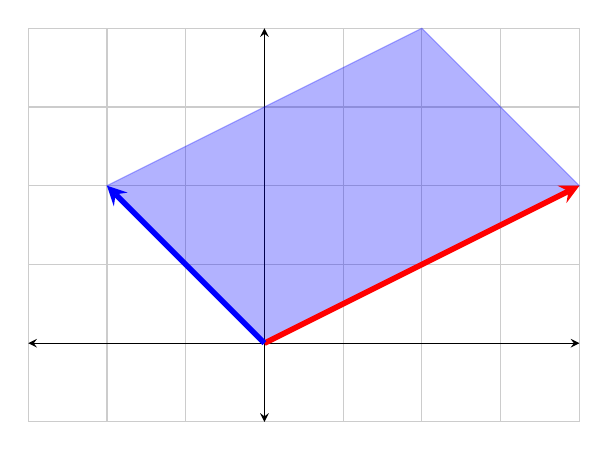
\begin{tikzpicture}[scale=1]
    \draw[thin,gray!40] (-3,-1) grid (4,4);
      \draw[<->] (-3,0)--(4,0);
      \draw[<->] (0,-1)--(0,4);
       
      \filldraw[blue, opacity=0.3](0,0)--(-2,2)--(2,4)--(4,2)--cycle;
     
    \draw[line width=2pt,red,-stealth](0,0)--(4,2);
     
     
     \draw[line width=2pt,blue,-stealth](0,0)--(-2,2);
      
    \end{tikzpicture}
    \end{center}
    \begin{explanation}
    The vectors that determine the parallelogram are
    $$\begin{bmatrix}4\\2\end{bmatrix}\quad\text{and}\quad\begin{bmatrix}-2\\2\end{bmatrix}$$
    The problem we run into is that these vectors are in $\RR^2$, whereas the cross product is defined only for vectors in $\RR^3$.  We will get around this difficulty by ``padding" our vectors with zeros on the bottom.  In other words, we will consider them as vectors sitting in the $xy$-coordinate plane in $\RR^3$.  This allows us to compute the cross product
    $$\begin{bmatrix}4\\2\\0\end{bmatrix}\times\begin{bmatrix}-2\\2\\0\end{bmatrix}=\begin{vmatrix}\vec{i}&\vec{j}&\vec{k}\\4&2&0\\-2&2&0\end{vmatrix}=\vec{k}\Big((4)(2)-(2)(-2)\Big)=12\vec{k}=\begin{bmatrix}0\\0\\12\end{bmatrix}$$
    The area of the parallelogram is then given by
    $$\mbox{Area}=\norm{\begin{bmatrix}0\\0\\12\end{bmatrix}}=12$$
    \end{explanation}
    \end{example}
     
    Example \ref{ex:areaofparallelogram} illustrates an important phenomenon.  Observe that the zeros in the last column of the determinant ensure that the $\vec{i}$ and $\vec{j}$ components of the cross product are zero, while the last component is the determinant of the $2\times 2$ matrix whose rows (or columns) are the two vectors that determine the parallelogram in $\RR^2$.  In general, if the parallelogram is determined by vectors
    $$\begin{bmatrix}a\\b\end{bmatrix}\quad\text{and}\quad\begin{bmatrix}c\\d\end{bmatrix}$$
    then the area of the parallelogram can be computed as follows:
    $$\begin{bmatrix}a\\b\\0\end{bmatrix}\times\begin{bmatrix}c\\d\\0\end{bmatrix}=\begin{vmatrix}\vec{i}&\vec{j}&\vec{k}\\a&b&0\\c&d&0\end{vmatrix}=\vec{k}\begin{vmatrix}a&b\\c&d\end{vmatrix}=\vec{k}\Big((a)(d)-(b)(c)\Big)=\begin{bmatrix}0\\0\\ad-bc\end{bmatrix}$$
     
    $$\mbox{Area}=\norm{\begin{bmatrix}0\\0\\ad-bc\end{bmatrix}}=|ad-bc|=\Big|\det\begin{bmatrix}a&b\\c&d\end{bmatrix}\Big|=\Big|\det\begin{bmatrix}a&c\\b&d\end{bmatrix}\Big|$$
     
    So the area of the parallelogram turns out to be the absolute value of the determinant of the matrix whose rows (or columns) are the two vectors that determine the parallelogram.
    The following formula summarizes our discussion.
     
    \begin{formula}\label{form:areaofparallelogramdeterminant} Let $\vec{u}=\begin{bmatrix}a\\b\end{bmatrix}$ and $\vec{v}=\begin{bmatrix}c\\d\end{bmatrix}$ be vectors of $\RR^2$.  The area of the parallelogram determined by $\vec{u}$ and $\vec{v}$ is given by
    $$\mbox{Area}=\Big|{\det\begin{bmatrix}a&b\\c&d\end{bmatrix}}\Big|=\Big|\det\begin{bmatrix}a&c\\b&d\end{bmatrix}\Big|$$
    \end{formula}
     
    \begin{example}\label{exp:polyArea}
        Use Formula \ref{form:areaofparallelogramdeterminant} to find the area of the polygon shown below.
      \begin{center}
    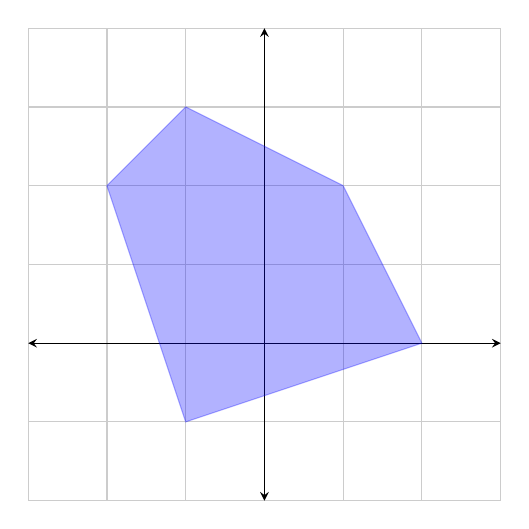
\begin{tikzpicture}[scale=1]
    \draw[thin,gray!40] (-3,-2) grid (3,4);
      \draw[<->] (-3,0)--(3,0);
      \draw[<->] (0,-2)--(0,4);
      \filldraw[blue, opacity=0.3](-1,-1)--(-2,2)--(-1,3)--(1,2)--(2,0)--cycle;
    %\draw[line width=2pt,red,-stealth](0,0)--(4,2);
    % \draw[line width=2pt,blue,-stealth](0,0)--(-2,2);
     \end{tikzpicture}
    \end{center} 
    \begin{explanation}
        We will start by splitting this region into triangles.
        \begin{center}
    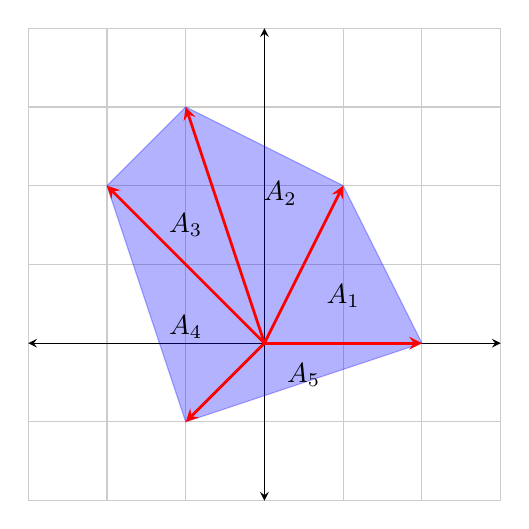
\begin{tikzpicture}[scale=1]
    \draw[thin,gray!40] (-3,-2) grid (3,4);
      \draw[<->] (-3,0)--(3,0);
      \draw[<->] (0,-2)--(0,4);
      \filldraw[blue, opacity=0.3](-1,-1)--(-2,2)--(-1,3)--(1,2)--(2,0)--cycle;
    \draw[line width=1pt,red,-stealth](0,0)--(-1,-1);
    \draw[line width=1pt,red,-stealth](0,0)--(-2,2);
    \draw[line width=1pt,red,-stealth](0,0)--(-1,3);
    \draw[line width=1pt,red,-stealth](0,0)--(1,2);
    \draw[line width=1pt,red,-stealth](0,0)--(2,0);
    \node[] at (1, 0.6)   (b) {$A_1$};
    \node[] at (0.2, 1.9)   (b) {$A_2$};
    \node[] at (-1, 1.5)   (b) {$A_3$};
    \node[] at (-1, 0.2)   (b) {$A_4$};
    \node[] at (0.5, -0.4)   (b) {$A_5$};
     \end{tikzpicture}
    \end{center}
        We can find the total area of the polygon by finding the area of each triangle.  The area of each triangle is half of the area of the corresponding parallelogram.  For instance, $A_1$ is half of the area of the parallelogram depicted below.
    \begin{center}
    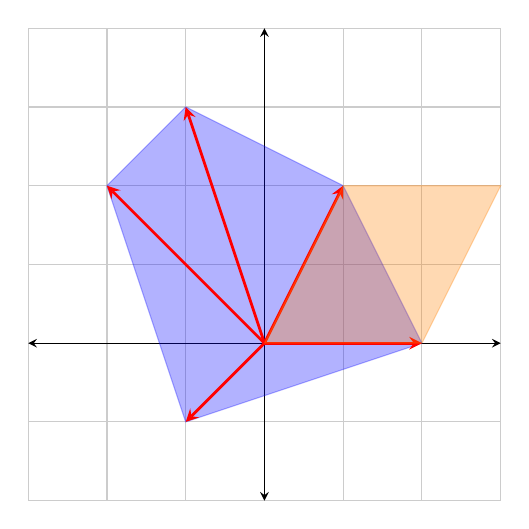
\begin{tikzpicture}[scale=1]
    \draw[thin,gray!40] (-3,-2) grid (3,4);
      \draw[<->] (-3,0)--(3,0);
      \draw[<->] (0,-2)--(0,4);
      \filldraw[blue, opacity=0.3](-1,-1)--(-2,2)--(-1,3)--(1,2)--(2,0)--cycle;
    \draw[line width=1pt,red,-stealth](0,0)--(-1,-1);
    \draw[line width=1pt,red,-stealth](0,0)--(-2,2);
    \draw[line width=1pt,red,-stealth](0,0)--(-1,3);
    \draw[line width=1pt,red,-stealth](0,0)--(1,2);
    \draw[line width=1pt,red,-stealth](0,0)--(2,0);
    \filldraw[orange, opacity=0.3](2,0)--(0,0)--(1,2)--(3,2)--cycle;
     \end{tikzpicture}
    \end{center}
    We compute
    $$A_1=\frac{1}{2}\left|\det\begin{bmatrix}2 & 1\\0 & 2\end{bmatrix}\right |=\answer{2}$$
    $$A_2=\frac{1}{2}\left|\det\begin{bmatrix}1 & -1\\2 & 3\end{bmatrix}\right |=\answer{2.5}$$
    $$A_3=\frac{1}{2}\left|\det\begin{bmatrix}-1 & -2\\3 & 2\end{bmatrix}\right |=\answer{2}$$
    $$A_4=\frac{1}{2}\left|\det\begin{bmatrix}-2 & -1\\2 & -1\end{bmatrix}\right |=\answer{2}$$
    $$A_5=\frac{1}{2}\left|\det\begin{bmatrix}-1 & 2\\-1 & 0\end{bmatrix}\right |=\answer{1}$$
    The total area of the polygon is $\answer{9.5}$.
    \end{explanation}
    \end{example}
     
     
    \subsection*{$3\times 3$ Determinant and the Volume of a Parallelepiped}
     
    Our next goal is to find the volume of a three-dimensional figure called a \dfn{parallelepiped}.  A parallelepiped is a six-faced figure whose opposite faces are congruent parallelograms located in parallel planes.  A parallelepiped is a three-dimensional counterpart of a parallelogram, and is determined by three non-coplanar vectors in $\RR^3$.  The figure below shows a parallelepiped determined by three vectors.
     
    \begin{center}
    \tdplotsetmaincoords{70}{130}
    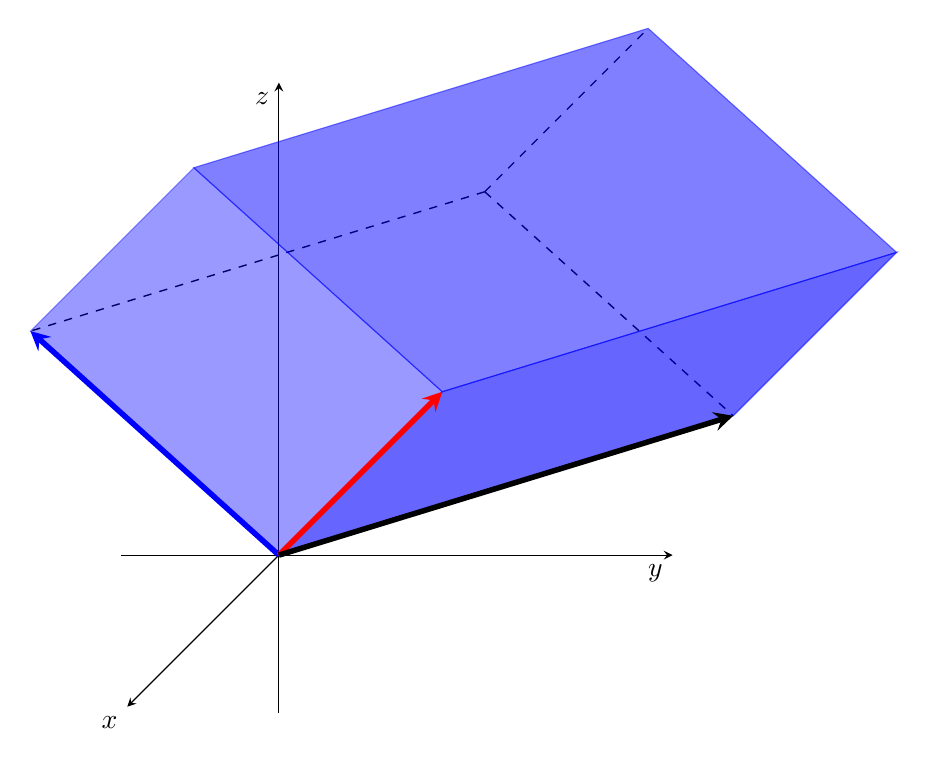
\begin{tikzpicture}
        \draw[->](-2,0,0)--(5,0,0) node[below left]{$y$};
        \draw[->](0,-2,0)--(0,6,0) node[below left]{$z$};
        \draw[->](0,0,-2)--(0,0,5) node[below left]{$x$};
         
        \draw[line width=0.5pt, dashed](3,5,1)--(5,1,-2);
        \draw[line width=0.5pt, dashed](3,5,1)--(-2,4,3);
        \draw[line width=0.5pt, dashed](3,5,1)--(7,9,6);
         
        \filldraw[blue, opacity=0.4] (0,0,0)--(-2, 4, 3)--(2,8,8)--(4,4,5)--cycle;
        \filldraw[blue, opacity=0.5] (2,8,8)--(4,4,5)--(9,5,3)--(7,9,6)--cycle;
        \filldraw[blue, opacity=0.6] (0,0,0)--(4,4,5)--(9,5,3)--(5,1,-2)--cycle;
         
        \draw[->, line width=2pt,blue, -stealth](0,0,0)--(-2,4,3);
        \draw[->, line width=2pt,red, -stealth](0,0,0)--(4,4,5);
        \draw[->, line width=2pt, -stealth](0,0,0)--(5,1,-2);
         
    \end{tikzpicture}
    \end{center}
     
    Consider a parallelepiped determined by vectors $\vec{u}$, $\vec{v}$ and $\vec{w}$, as shown below. 
     
    \begin{center}
    \tdplotsetmaincoords{70}{130}
    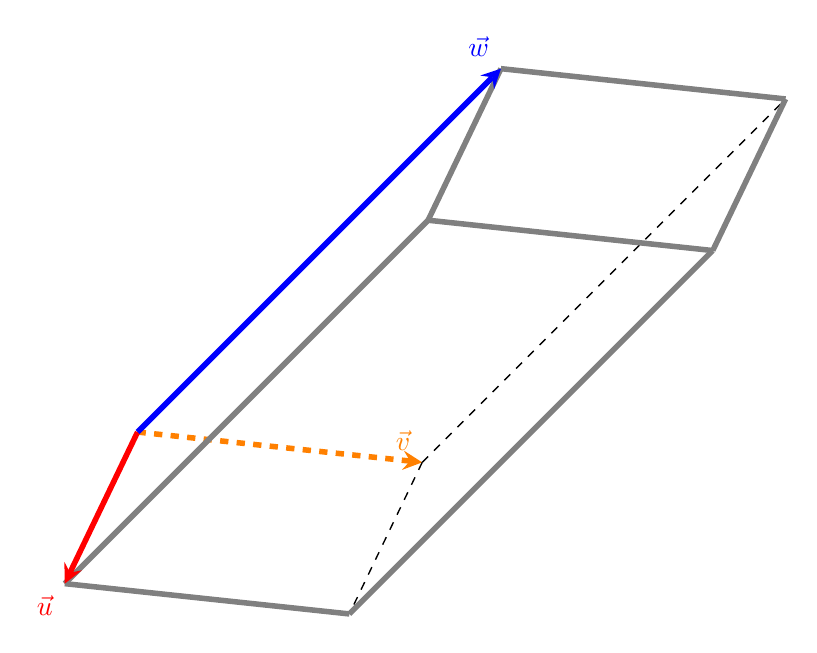
\begin{tikzpicture}
        \draw[->, line width=2pt, -stealth,orange,dashed](0,0,0)--(4,0,1)node[above left]{$\vec{v}$};
         
        \draw[line width=0.5pt, dashed](4,0,1)--(5,0,6);
        \draw[line width=0.5pt, dashed](4,0,1)--(9,5,2);
         
        \draw[line width=2pt, gray](1,0,5)--(6,5,6);
        \draw[line width=2pt, gray](10,5,7)--(6,5,6);
        \draw[line width=2pt, gray](10,5,7)--(5,0,6);
        \draw[line width=2pt, gray](1,0,5)--(5,0,6);
        \draw[line width=2pt, gray](6,5,6)--(5,5,1);
        \draw[line width=2pt, gray](9,5,2)--(5,5,1);
        \draw[line width=2pt, gray](10,5,7)--(9,5,2);
         
        \draw[->, line width=2pt,red, -stealth](0,0,0)--(1,0,5)node[below left]{$\vec{u}$};
        \draw[->, line width=2pt, blue, -stealth](0,0,0)--(5,5,1)node[above left]{$\vec{w}$} ;
       
    \end{tikzpicture}
    \end{center}
     
    The volume of a parallelepiped is given by
    $$\mbox{Volume}=(\text{area of base})(\text{height})$$
    We will consider the parallelogram determined by $\vec{u}$ and $\vec{v}$ to be the base of the parallelepiped.  Thus, the area of the base is given by
    $$\mbox{Area of Base}=\norm{\vec{u}\times\vec{v}}$$
    \begin{center}
    \tdplotsetmaincoords{70}{130}
    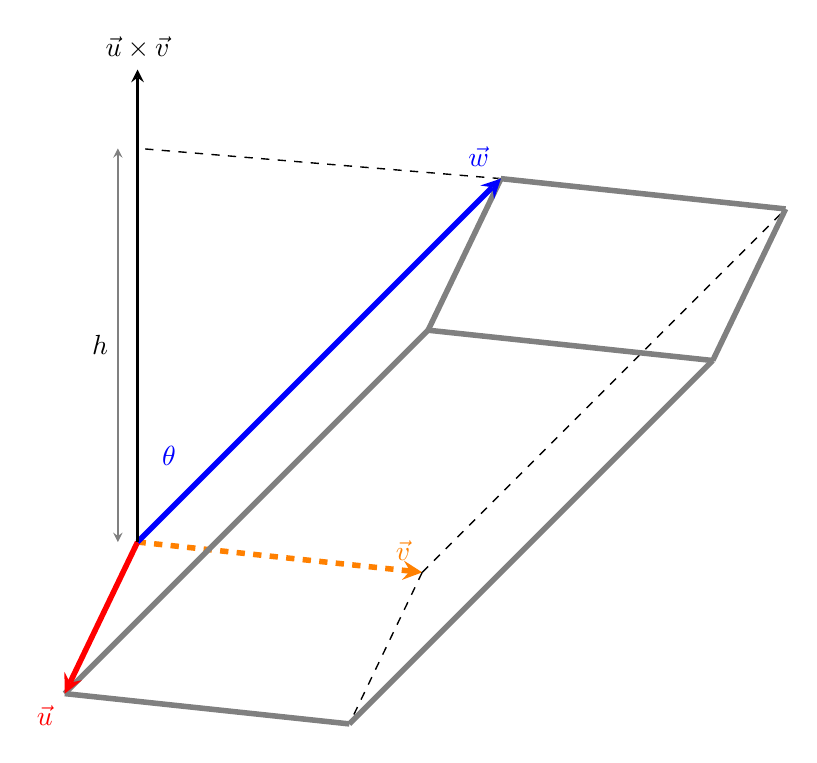
\begin{tikzpicture}
        \draw[->, line width=2pt, -stealth,orange,dashed](0,0,0)--(4,0,1)node[above left]{$\vec{v}$};
         
        \draw[line width=0.5pt, dashed](4,0,1)--(5,0,6);
        \draw[line width=0.5pt, dashed](4,0,1)--(9,5,2);
         
        \draw[line width=0.5pt, dashed](5,5,1)--(0,5,0);
         
        \draw[line width=2pt, gray](1,0,5)--(6,5,6);
        \draw[line width=2pt, gray](10,5,7)--(6,5,6);
        \draw[line width=2pt, gray](10,5,7)--(5,0,6);
        \draw[line width=2pt, gray](1,0,5)--(5,0,6);
        \draw[line width=2pt, gray](6,5,6)--(5,5,1);
        \draw[line width=2pt, gray](9,5,2)--(5,5,1);
        \draw[line width=2pt, gray](10,5,7)--(9,5,2);
         
        \draw[->, line width=2pt,red, -stealth](0,0,0)--(1,0,5)node[below left]{$\vec{u}$};
        \draw[->, line width=2pt, blue, -stealth](0,0,0)--(5,5,1)node[above left]{$\vec{w}$} ;
        \node[blue] at (0.4, 1.1)   (b) {$\theta$};
        \draw[->, line width=1pt, -stealth](0,0,0)--(0,6,0) node[above]{$\vec{u}\times\vec{v}$};
        \draw[->, gray, line width=0.5pt, -stealth](-0.25,2.5,0)node[left, black]{$h$}--(-0.25,0,0);
        \draw[->, gray, line width=0.5pt, -stealth](-0.25,2.5,0)--(-0.25,5,0);
    \end{tikzpicture}
    \end{center}
     
    The height of the parallelepiped is measured along a line perpendicular to the base.  By Theorem \ref{th:crossproductorthtouandv}, $\vec{u}\times\vec{v}$ lies on such a line.  Let $\theta$ be the angle between $\vec{w}$ and $\vec{u}\times\vec{v}$, $0\leq \theta\leq\pi$.  Then the height, $h$, of the parallelepiped is given by
    $$h=\norm{\vec{w}}|\cos\theta |$$
     
    It may be difficult to visualize this in two dimensions.  Below is a replica of of the above diagram in GeoGebra.  RIGHT-CLICK and DRAG to rotate the image.
     
    \pdfOnly{
    Access GeoGebra interactives through the online version of this text at
     
    \href{https://ximera.osu.edu/oerlinalg}{https://ximera.osu.edu/oerlinalg}.
    }
     
    \begin{onlineOnly}
    \begin{center}
    \geogebra{tfuzeqwr}{900}{700}
    \end{center}
    \end{onlineOnly}
     
    This gives us the following formula for the volume of the parallelepiped
    $$\mbox{Volume}=\norm{\vec{u}\times\vec{v}}\norm{\vec{w}}|\cos\theta |=|(\vec{u}\times\vec{v})\dotp\vec{w}|$$
     
    We have established the following formula.
     
    \begin{formula}\label{form:volumeparallelepiped}
    The volume of a parallelepiped determined by vectors $\vec{u}$, $\vec{v}$ and $\vec{w}$ in $\RR^3$ is given by\\
    $$\mbox{Volume}=|(\vec{u}\times\vec{v})\dotp\vec{w}|$$
    \end{formula}
     
    Our next goal is to show that this expression for the volume is equal to the determinant of a $3\times 3$ matrix whose rows are the vectors that determine the parallelepiped.
     
    Let
    $$\vec{u}=\begin{bmatrix}u_1\\u_2\\u_3\end{bmatrix},\quad\vec{v}=\begin{bmatrix}v_1\\v_2\\v_3\end{bmatrix},\quad\vec{w}=\begin{bmatrix}w_1\\w_2\\w_3\end{bmatrix}$$
    then
    \begin{align}\label{eq:boxproduct}(\vec{u}\times\vec{v})\dotp\vec{w}=\begin{vmatrix}\vec{i}&\vec{j}&\vec{k}\\u_1&u_2&u_3\\v_1&v_2&v_3\end{vmatrix}\dotp\begin{bmatrix}w_1\\w_2\\w_3\end{bmatrix}=\begin{vmatrix}w_1&w_2&w_3\\u_1&u_2&u_3\\v_1&v_2&v_3\end{vmatrix}
    \end{align}
    The expression in (\ref{eq:boxproduct}) is sometimes referred to as the \dfn{box product} or the \dfn{scalar triple product}.
     
    Recall that $\det(A)=\det(A^T)$ (Theorem \ref{th:detoftrans}).  Therefore, the three vectors that determine the parallelogram can be used to form rows or columns of the determinant on the right side of (\ref{eq:boxproduct}).  This gives us the following formula.
     
    \begin{formula}\label{form:boxproduct}
    Let $\vec{u}=\begin{bmatrix}u_1\\u_2\\u_3\end{bmatrix},\quad\vec{v}=\begin{bmatrix}v_1\\v_2\\v_3\end{bmatrix},\quad\vec{w}=\begin{bmatrix}w_1\\w_2\\w_3\end{bmatrix}$ be vectors in $\RR^3$.  Then the volume of the parallelepiped determined by $\vec{u}$, $\vec{v}$ and $\vec{w}$ is given by
    $$\mbox{Volume}=\Big|\det\begin{bmatrix}w_1&w_2&w_3\\u_1&u_2&u_3\\v_1&v_2&v_3\end{bmatrix}\Big|=\Big|\det\begin{bmatrix}w_1&u_1&v_1\\w_2&u_2&v_2\\w_3&u_3&v_3\end{bmatrix}\Big|$$
    \end{formula}
     
    \subsection*{Determinants and Linear Transformations}
    We will now turn our attention to the determinant of a matrix of a linear transformation. 
     
    \begin{exploration}\label{exp:LinTransAreaDet}
    The following GeoGebra interactive shows a polygon $P$ located in the domain of a linear transformation $T$ induced by the matrix $M$.  The right-hand side shows the image of $P$ under $T$.  The number inside each polygon indicates its area.
     
    \pdfOnly{
    Access GeoGebra interactives through the online version of this text at
     
    \href{https://ximera.osu.edu/oerlinalg}{https://ximera.osu.edu/oerlinalg}.
    }
     
    \begin{onlineOnly}
    \begin{center}
    \geogebra{nr8jsz4w}{950}{700}
    \end{center}
    \end{onlineOnly}
     
    \begin{question}
    Let $M=\begin{bmatrix}1&1\\-1&2\end{bmatrix}$.  Find the determinant of $M$.
    $$\det{M}=\answer{3}$$
    Drag the vertices of $P$ to change the polygon.  Make a note of how the area of $P$ and the area of the image change.  How are the areas related to each other?
    $$\mbox{Area}(T(P))=\answer{3}\mbox{Area}(P)$$
    \end{question}
    \begin{question}
    Change the matrix $M$ to a matrix whose determinant is 1.  Compare the areas of $P$ and $T(P)$.  Try matrices whose determinant is 0 or negative.  What do you observe about the areas?
     
    Formulate a conjecture about the relationship between the area of the polygon and the area of its image under a linear transformation.
    \end{question}
    \end{exploration}
    We will not prove your conjecture in Exploration \ref{exp:LinTransAreaDet} for arbitrary figures as it is beyond the scope of this text.  However, we can tackle the problem of how linear transformations affect areas of parallelograms.  This is the topic of our next example.
     
    \begin{example}\label{ex:detLinTransArea}
        Let $T:\RR^2\longrightarrow\RR^2$ be a linear transformation induced by matrix $M$.  Suppose $\vec{u}$ and $\vec{v}$ are vectors in $\RR^2$.  Let $P$ be a parallelogram determined by $\vec{u}$ and $\vec{v}$.  Show that
        $$\mbox{Area}(T(P))=\left|\det{M}\right|\mbox{Area}(P)$$
        \begin{explanation}
            Let $\vec{u}=\begin{bmatrix}a\\b\end{bmatrix}$ and $\vec{v}=\begin{bmatrix}c\\d\end{bmatrix}$, and let $M=\begin{bmatrix}m & n\\p & q\end{bmatrix}$.  By Formula \ref{form:areaofparallelogramdeterminant}, $\mbox{Area}(P)=ad-bc$.  Applying $M$ to $\vec{u}$ and $\vec{v}$ we get
            $$T(\vec{u})=\begin{bmatrix}am+bn\\ap+bq\end{bmatrix}\quad\mbox{and}\quad T(\vec{v})=\begin{bmatrix}cm+dn\\cp+dq\end{bmatrix}$$
            Using Formula \ref{form:areaofparallelogramdeterminant}, we compute
            \begin{align*}
            \mbox{Area}(T(P))=&|(am+bn)(cp+dq)-(ap+bq)(cm+dn)|\\
            =&|(mq-np)(ad-bc)|\\
            =&|\det{M}|\mbox{Area}(P)
            \end{align*}
        \end{explanation}
    \end{example}
     



\end{document}